\begin{frame}{Introduction}
\lowEmph{Data-flow analysis} plays an important role in software development, and helps developers to detect subtle bugs
% :
%	\begin{itemize}
%		\item \lowEmph{Null-pointer dereferencing}
%		\item \lowEmph{Dead Assignment}
%	\end{itemize}

\onslide<2->{
\begin{center}
\emphSlide{ Source-level dataflow analysis ... why  ?}
\end{center}
	\begin{itemize}
	\item Easier integration with IDE
	\item Reports are directly linked to the source code
%	\item What many commercial tools do, e.g., SonarQube, ErrorProne, ...
	\end{itemize}
}
\onslide<3->{
\begin{center}
\emphSlide{The main challenges were:}
\end{center}
		\begin{itemize}
			\item Large engineering effort for each source language
			\item The syntax doesn't always reflect the program's semantics
		\end{itemize}
}
\end{frame}


\begin{frame}{Our approach}
	We build the CFGs as extension of the AST using Reference Attribute Grammars (RAGs)\\ \vspace{0.1cm}
	\begin{itemize}
		\item \lowEmph{Declarative} specification \\ \vspace{0.1cm}
		\item Handle \lowEmph{implicit control flow} \\ \vspace{0.1cm}
		\item Overcome the limitations of an earlier framework \\ \vspace{0.1cm}
	\end{itemize}

\begin{center}
	\emphSlide{Research questions}
\end{center}

	\begin{itemize}
		\item How  can we reduce the engineering effort ? \\ \vspace{0.1cm}
		\item How can we fill the gap between \textit{syntax and semantics} ? \\ \vspace{0.1cm}
		\item Is our new approach competitive performance-wise?    \\ \vspace{0.1cm}
	\end{itemize}
\end{frame}

\begin{frame}{Intraprocedural RAG-based CFGs}
\begin{center}
	We removed the limitations of the previous approach

	\only<1>{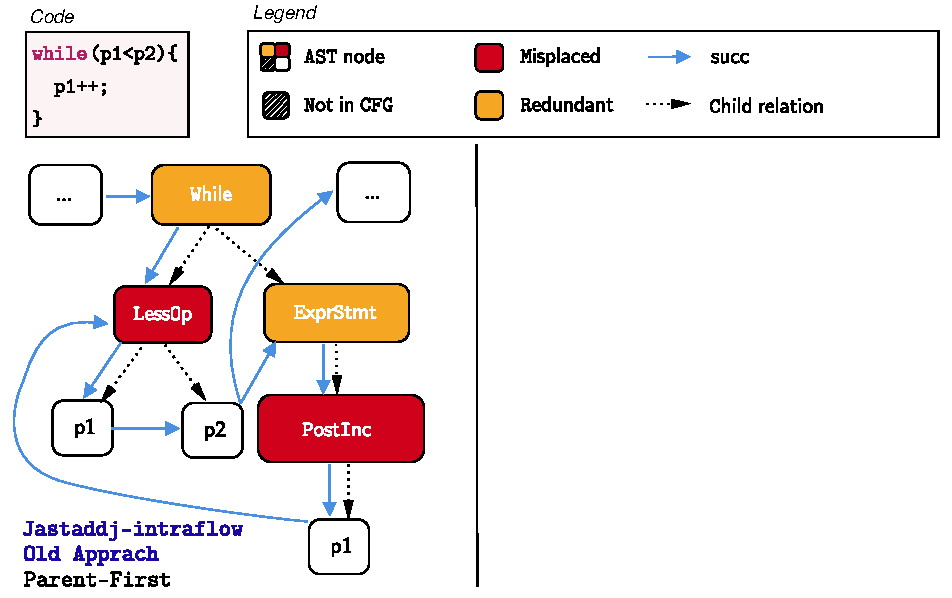
\includegraphics[scale=0.60]{img/intro2.pdf}}%
    \only<2>{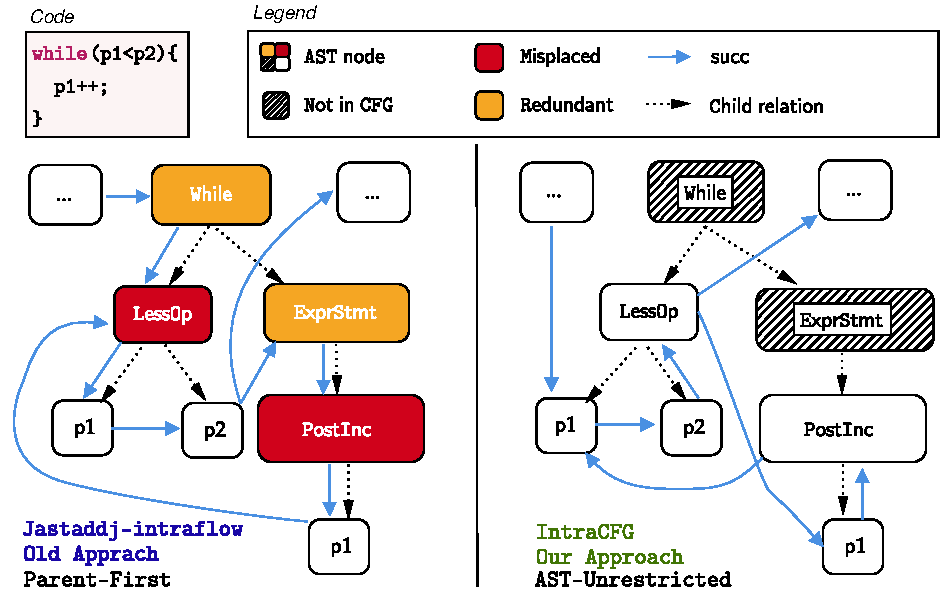
\includegraphics[scale=0.60]{img/intro1.pdf}}%
\end{center}

\end{frame}


\begin{frame}{Modular architecture}
	\hspace*{-0.9cm}
	\only<1>{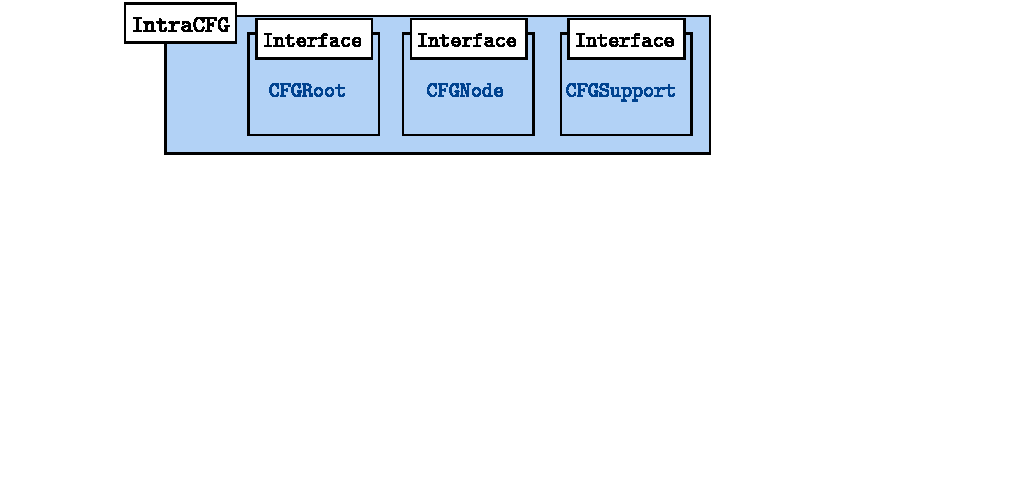
\includegraphics[scale=0.73]{img/ModularArchitecture1.pdf}}%
	\only<2>{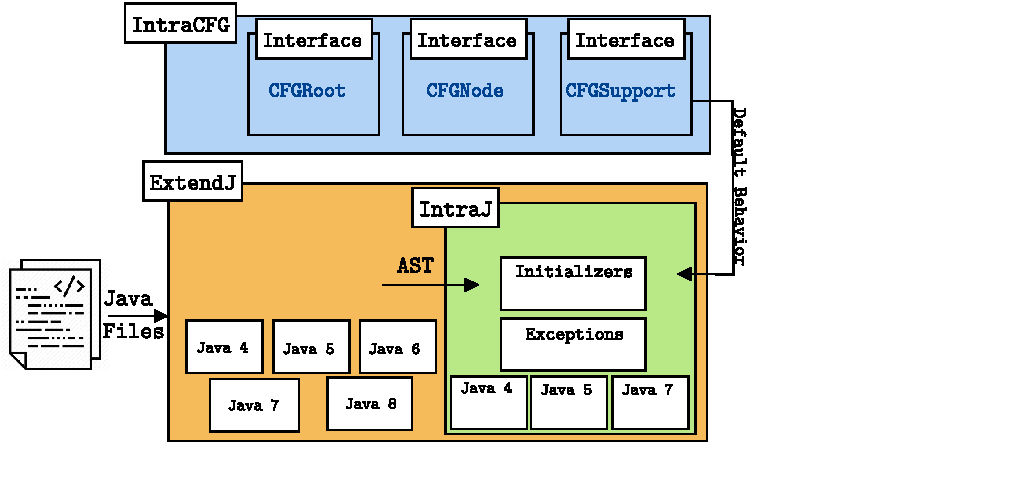
\includegraphics[scale=0.73]{img/ModularArchitecture2.pdf}}%
	\only<3>{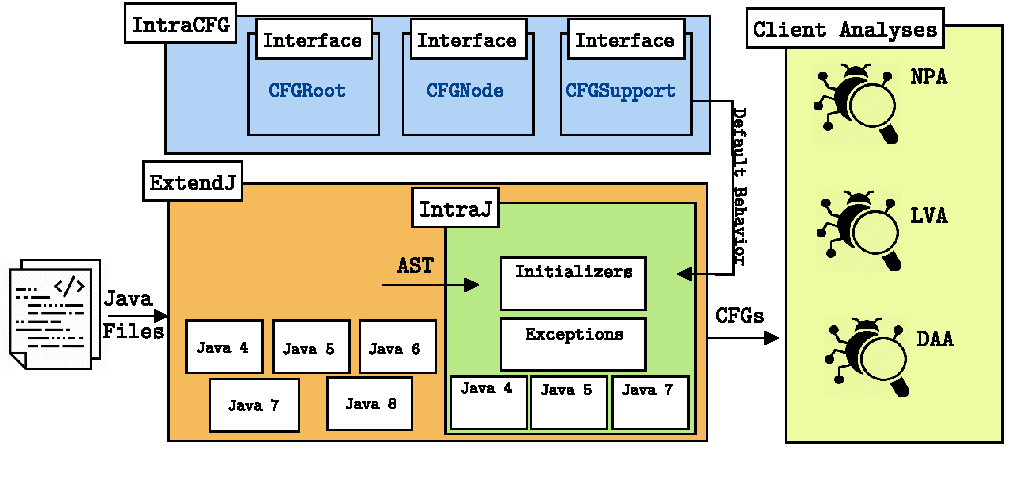
\includegraphics[scale=0.73]{img/ModularArchitecture3.pdf}}%
	\only<4>{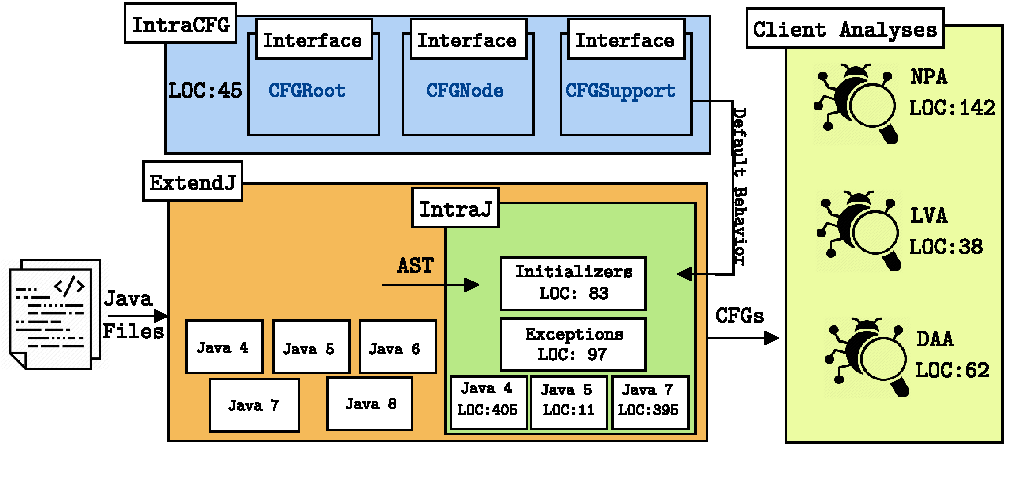
\includegraphics[scale=0.73]{img/ModularArchitecture4.pdf}}%
\end{frame}




